\chapter{Platform Design and Implementation}

As we mentioned in Chapter 1, the goal of this thesis was to develop an
interface for reinforcement learning research in StarCraft. The following
sections outline the process of design, implementation and testing of the
platform.

\section{Specifications}

Obtaining a list of specifications for the platform was relatively challenging
for a few reasons: the design needed to provide a powerful and robust
environment while maintaining a strong degree of expandability. With the sudden
re-popularisation of reinforcement learning the community has begun challenging
previously untouched problems, meaning that entirely new architectures might
soon appear and provide new constraints for existing platforms.

We identified the following minimal requirements:

\begin{itemize}
\item Ability to control StarCraft. This included (but was not limited to)
  starting, pausing, and ending games, killing and re-starting the program,
  selecting certain maps or campaigns.
\item Ability to collect and share game state information.
\item Ability to control the game from the player perspective
\item Ability to collect data from human players and replays available over the
  internet.
\item Ability to use hacks and / or some of the cheats to deactivate some of the
  features that make the general game particularly hard (e.g. fog of war).
\end{itemize}

Additionally the surge of deep reinforcement learning gave us an important
additional requirement: we would need to provide a way to use one or some of the
currently popular deep learning libraries, and a native interface to the visual
output of the game.

\section{Brood War Application Program Interface}

One of the main reasons this project became possible within the given time
constraint was because of the existence of the Brood War Application Program
Interface (BWAPI) \citep{bwapi2011brood}. A closed-source game like StarCraft
would normally be very hard to control and to use as an AI development
framework, but thanks to a few extraordinary developers since 2009 it has been
possible to build bots for the game. BWAPI provides a clean and modular
interface that provides access to the game data structures, allowing to collect
game information and to control units much in the same way a human player would.
Because of its C++ implementation, it's also optimised for speed, however its
design model makes it unfortunately thread-unsafe.

BWAPI uses DLL injection to interact with the game, providing two interfaces to
the game: BWAPIModule and BWAPIClient. The first one allows to control of the
units through callbacks fired by in-game events, so it's mostly suitable for
running agents that do not require to have complete control over the game (as
the game is configured centrally by the injected BWAPI.dll at startup). The
second interface allows to directly connect and interact with the server started
within BWAPI.dll, which gives the ability to arbitrarily control most of the
process state. Even thought BWAPIClient lacked some documentation, we decided to
use it to give us the maximum amount of maneuverability later in the
implementation phase.

\section{Pipeline Design} % 2 pages ()

StarCraft and BWAPI by default are only supported on Windows platforms (We
tested Windows 7, 8 and 10), but most of the critical machine learning and
tensor libraries are actively developed only on Unix systems. While the
situation has gradually seen some improvements with the introduction of CNTK
\citep{dallycntk} and TensorFlow \cite{abaditensorflow} (available on Windows
through Docker), most of the current state-of-the-art development and research
happens on Torch, Theano and Caffe, most of which are widely supported only on
Linux and OS X. Given these constraints we decided to separate our system in two
parts: one running on Windows and directly communicating with StarCraft, and the
other running on Linux and interfacing with one of the mentioned tensor
libraries.

\begin{figure}[h]
    \centering
    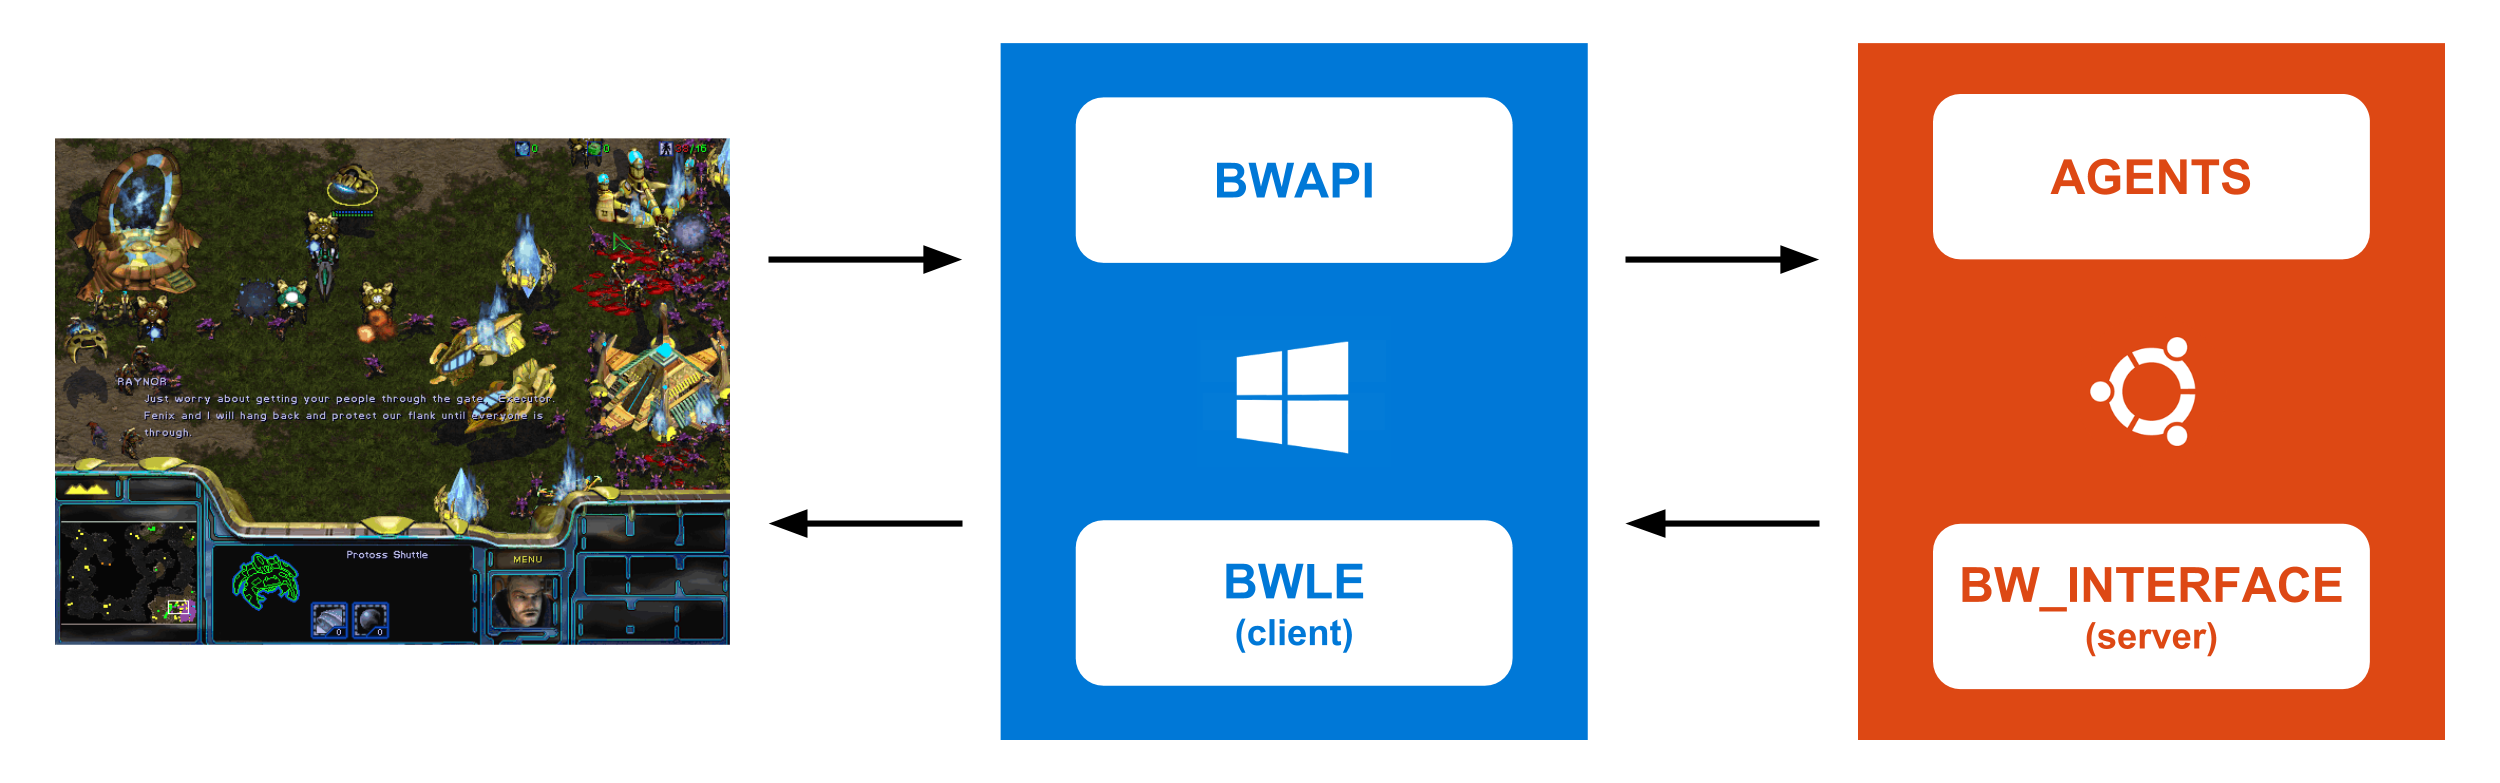
\includegraphics[width=\textwidth]{ch3/arch_overall}
    \caption{Overall architecture. The interface running on Windows 7
      communicates with StarCraft using BWAPI, and connects to a Linux server
      using standard non-blocking sockets. The Linux interfaces communicates
      with an agent through shared objects, }
    \label{fig:arch_ov}
\end{figure}

We designed the systems to communicate between each other using non-blocking TCP
sockets in a synchronous or asynchronous fashion depending on the interface-wide
configuration settings. The choice is dependent mostly on the targeted
experimental setting:

\begin{itemize}
\item synchronous communication can be used to simulate the standard MDP-like
  setting where at each step all agents receive the entirety of all observable
  data, the environment is blocked until the decision process has finished, and
  the environment executes a step when the MDP processes send a certain command.
\item asynchronous communication is instead more useful to have a closer
  simulation to real-world scenarios and games. In this mode the game executes
  each step at a fixed rate and sends information as fast as possible (as the
  game steps rate can be much faster than it's currently possible to process and
  send the visual data). The agent can then send actions at any point of the
  process, which are then executed in the next immediate step.
  This mode is significantly more challenging.
\end{itemize}

To be as efficient and fast as possible, the data structures containing the game
information are serialised using the Google protobuf library
\citep{varda2008protocol}. The library provides a way to generate serialised
objects using pre-defined schemas, which can then be filled with game
information and sent over as compressed strings. Unfortunately the library is
not optimised for very large objects, so in addition to it we implemented our
own serialisation method for sending the image structure over the socket
interface.

While both systems are fully functional, the asynchronous interface requires a
significant amount of work on the agent side to sync the data sources and take
into account the perception/action delay. Such processes are generally
considered a source of research problems but they are not of great interest to
decision making, as once the system is modelled it just becomes part of the
environment.

For the sake of clarity and brevity we will therefore from now on describe the
rest of the system only with respect to the synchronous communication system, as
the implementation of the rest of the modules is mostly independent from this
choice and it greatly simplifies the explanation of the agent interface.

\subsection{Windows Interface}

\begin{figure}[h]
    \centering
    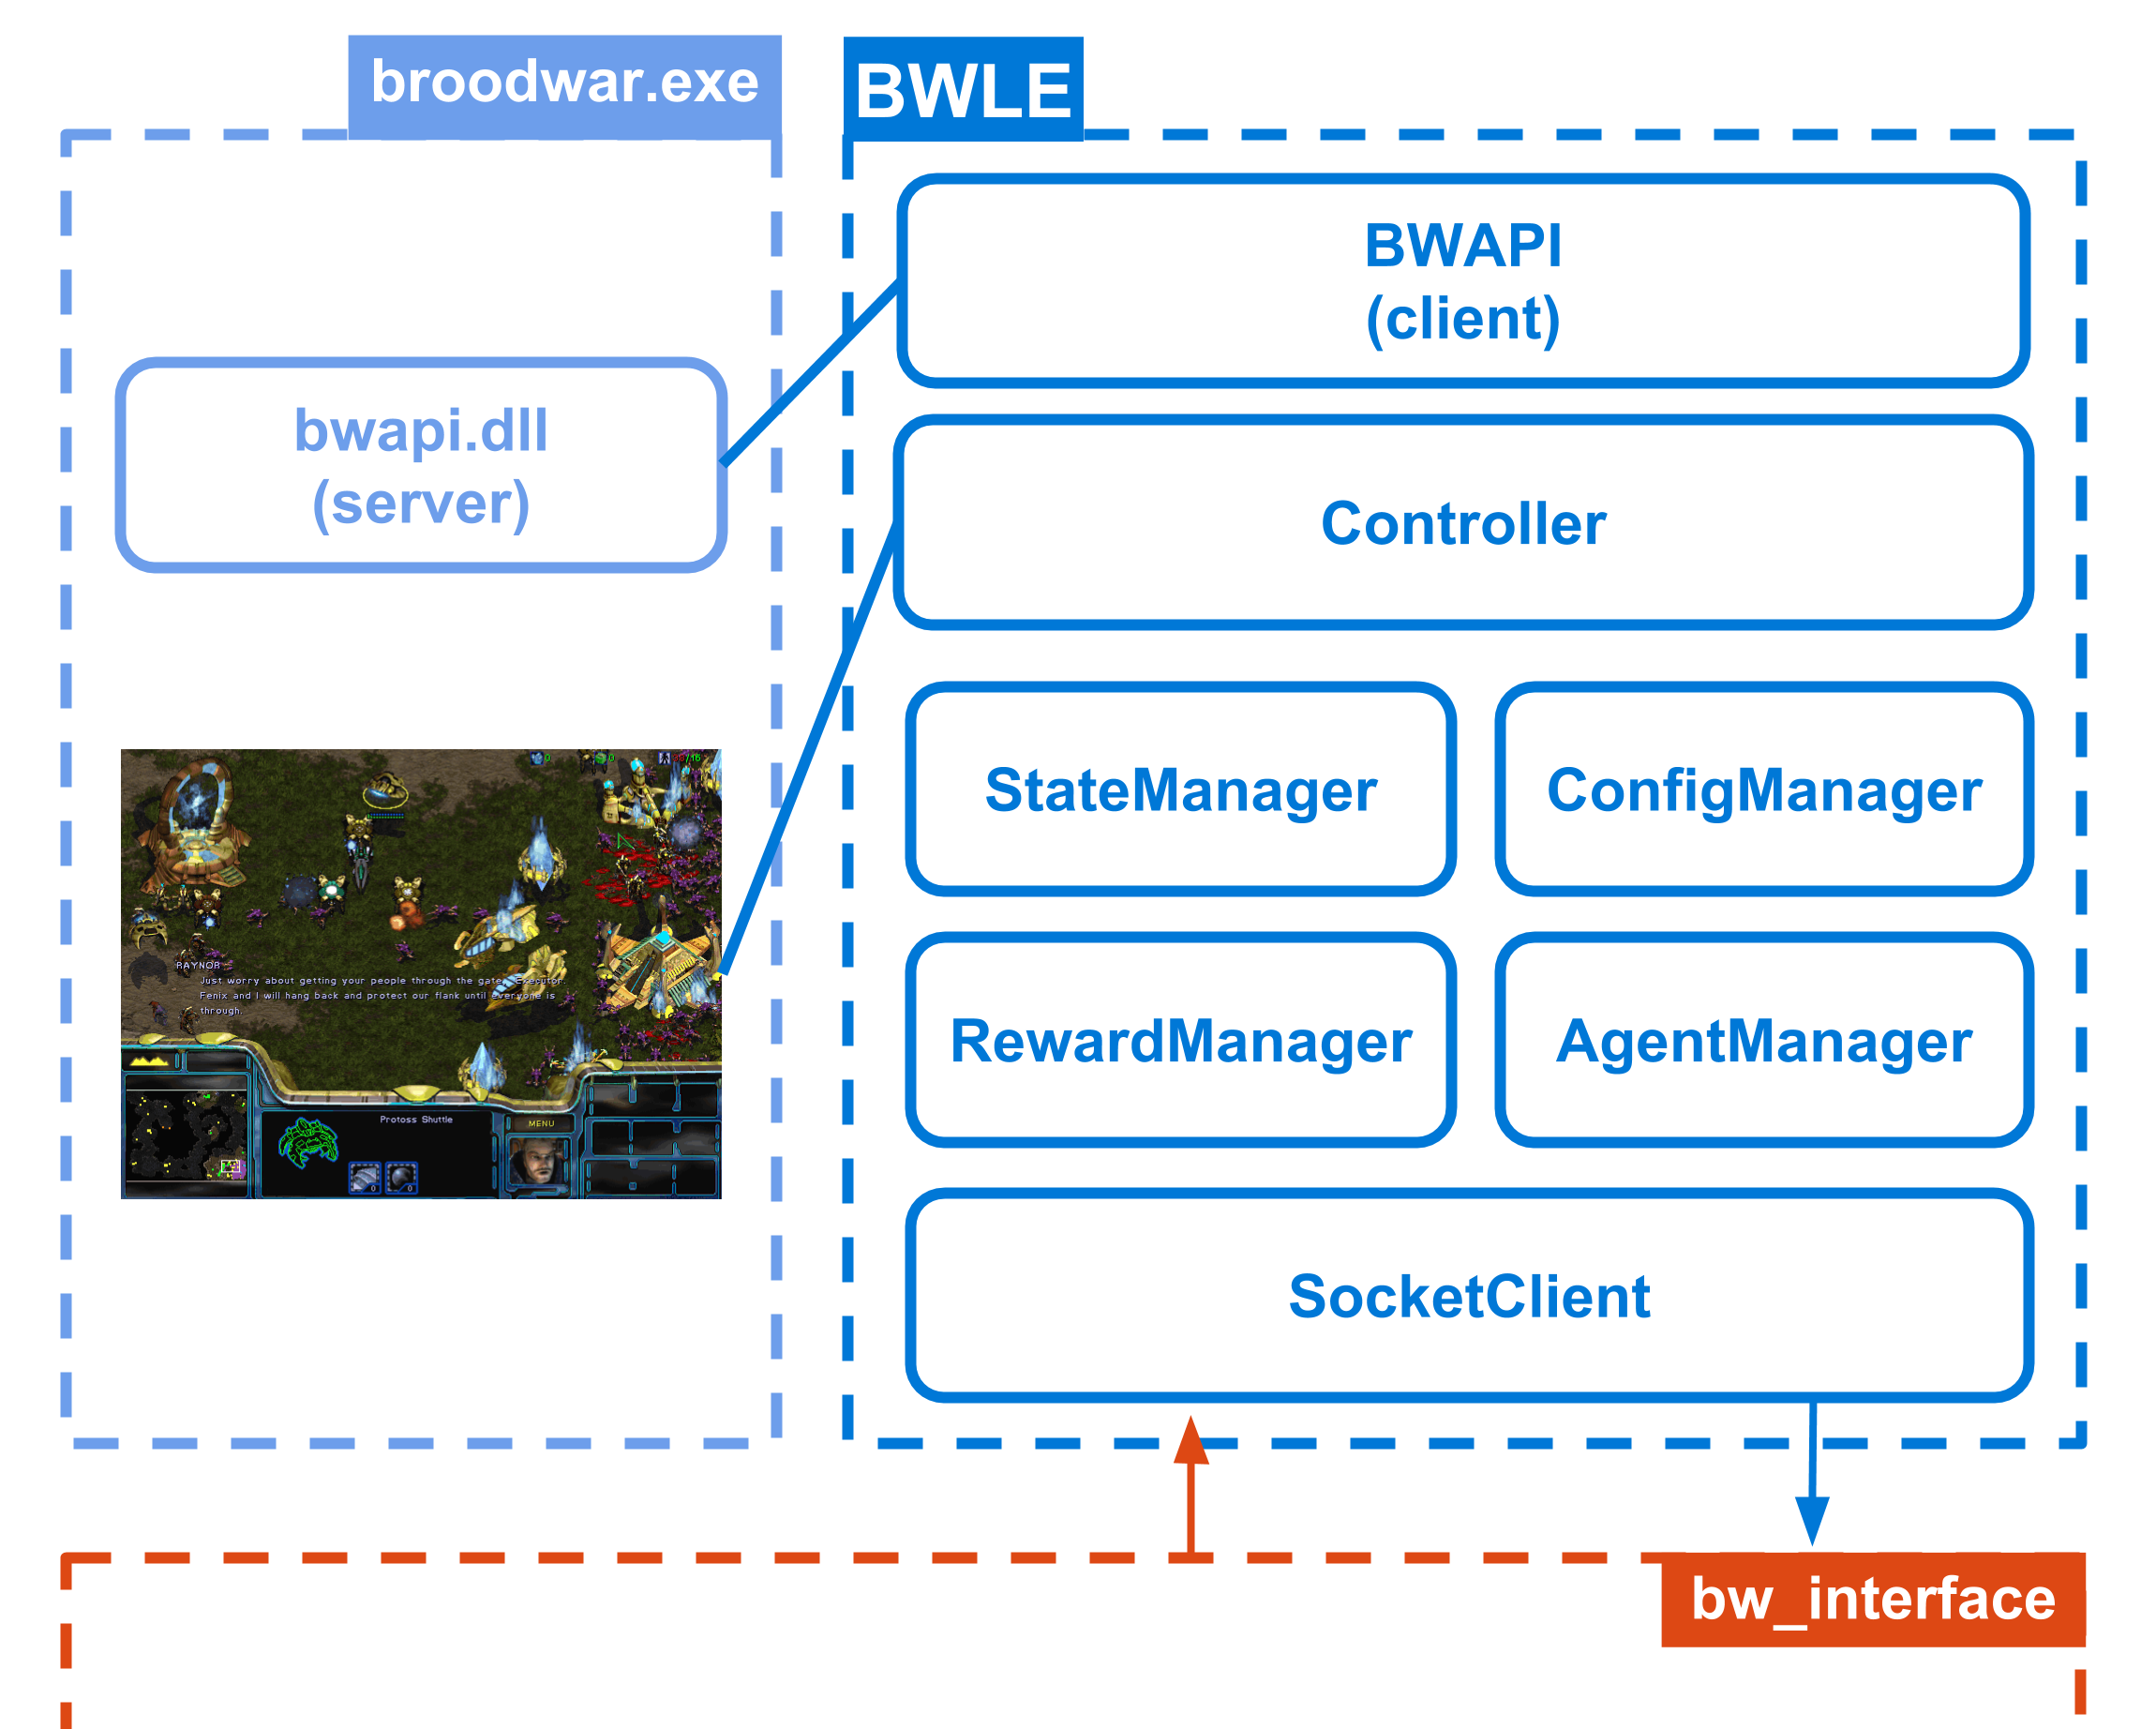
\includegraphics[width=\textwidth]{ch3/arch_win}
    \caption{Overview of the architecture on the Windows sub-system.}
    \label{fig:arch_win}
\end{figure}

To avoid any compatibility problems and to be as fast as possible, we
implemented this side of the architecture in C++ using Windows' Visual C++
compiler. The interface, called \texttt{Brood War Learning Environment} (BWLE)
automatically starts the game, injects \texttt{BWAPI.ddl} and tries to connect
to one of the servers specified in the configuration file(s).

\subsubsection{StarCraft Controller}

Games can be interrupted, terminated or restarted at any time. The client allows
to either completely kill StarCraft, therefore resetting its state with a
process-wide restart, or to just use the in-game restart function to quit the
game and start a new one. The first method allows to change certain settings
that can be loaded only when StarCraft is started, but stops BWAPI for around
two seconds on a quad-core machine between issuing the kill command and the
first step of a new game. The second method allows instead to start a new game
in less than a second. % CITATION NEEDED (check starcraft times)

\begin{sflisting}[caption=Example of a BWLE's configuration file. Fields are not
  mandatory and have reasonable default values. Most of the available options
  are not shown., label=ls:config] 
[standard]
port=12312
address=192.168.0.1
with_image=true
image_skip=0
reward_mode=0
turn_skip=10
map_file=..\share\maps_test_up.txt
map_mode=random
\end{sflisting}

BWLE's configuration system has been written to parse standard INI files,
focusing on completely hiding BWAPI and presenting a unique and coherent
configuration system with useful defaults. A list of maps can then be load in
the system by specifying a file containing a list of files or directories. The
game can also be set to load maps sequentially or in random order, which is an
essential feature for standard training procedures. All the random processes
within BWAPI and the interface can be controlled by specifying a seed at the
start of the experiment. An example configuration can be seen in Listing
\ref{ls:config}.

% TODO: add seed to game if possible, otherwise future work

\subsubsection{Screen capturing}

% TODO describe window size

BWAPI does not provide any interface to capture the visual output of the
game\footnote{Some work had been previously done to integrate some form of
  streaming functionality within BWAPI, but it was dropped in favour of existing
  tools. See https://github.com/bwapi/bwapi/issues/596}, so to fulfill the
specification we developed a module to capture the StarCraft window and include
it in the game state.

To achieve this functionality we use the Graphics Device Interface library
Gdiplus - included as part of the standard Windows Software Development Kit - to
find the StarCraft process, grab an handler to its window, and extract the raw
pixel data. The obtained data structure stores the pixel in an array of 32bit
integers, where integer represent the row-wise RGB data and a null byte.

\begin{figure}[h]
    \centering
    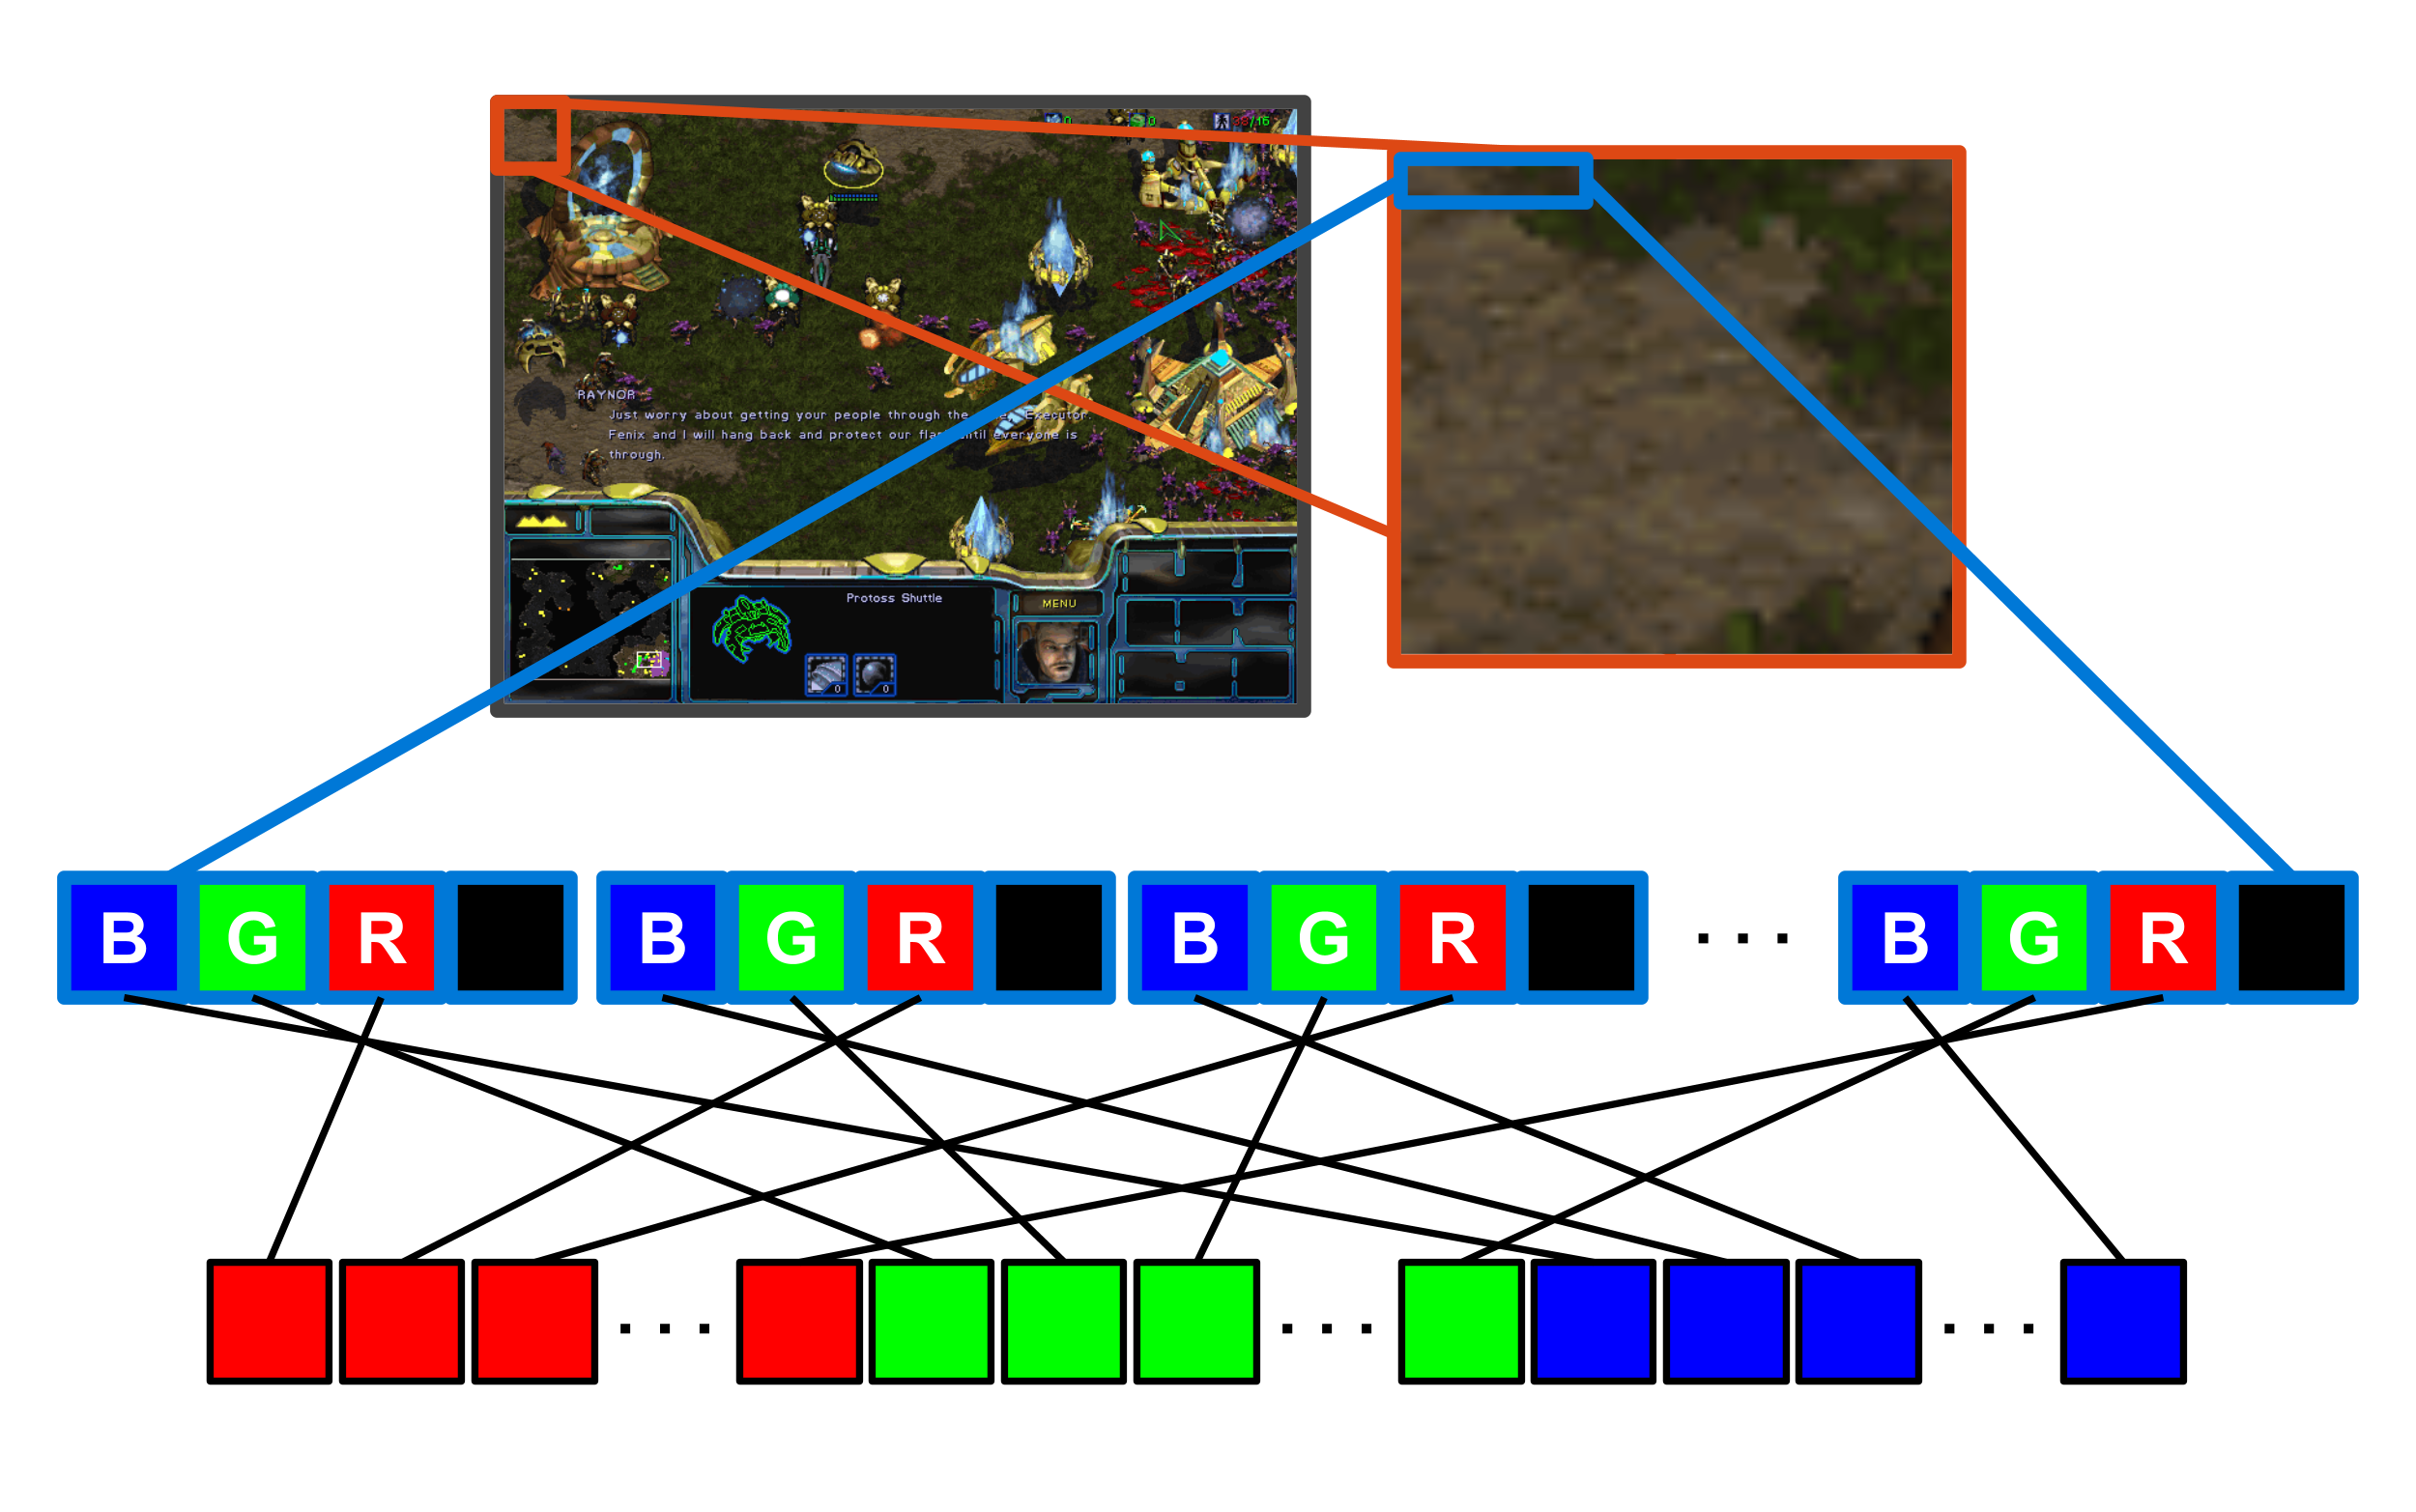
\includegraphics[width=\textwidth]{ch3/capt_conv}
    \caption{Conversion process of the visual data. The raw pixel data captured
      using the window handler gets stripped of superfluous data and separated
      by channel at the same time.}
    \label{fig:capt_conv}
\end{figure}

Before serialising the data to use the network endianness order over the wire,
we strip the null byte and we cluster the channels separately to obtain first
all the red channel values, then the gree channel values, and finally the blue
channel values (Figure \ref{fig:capt_conv}). It must be noted that while this
process has been made as fast as possible on the single thread (given the frame
size), it could be even further optimised by exploiting the fact that the
channels are essentially already independent. 

To allow BWLE to modify the size of the window at running-time we stored all the
captured data using dynamic-size arrays. This required us to add information
such as windows size and bit-dept to the game state data structure so that the
server would be able to calculate the image buffer without making mistakes and
corrupting the data.

% TODO describe image serialisation

\subsubsection{Collecting the Game State}

Collecting the game state also represented a non-trivial design and
implementation challenge. BWAPI was designed with the idea of writing classical
AI bots, not general learning systems. This essentially meant having to deal
with a purposely modular interface split into different objects with respect to
unit classes, weapons, available upgrades, events, forces and so on. The process
of developing a module to collect the game state in a straightforward manner
ended up consisting into many hours of development and testing to learn most of
BWAPI's large functionality. The final outcome was a modifiable query class
\texttt{StateManager} that walks most of the available internal interface while
filtering out errors and unneeded information. Once the module has obtained the
game state, the entirety of the data is loaded into a protobuffer so that it can
be sent over the wire and parsed by the server running on the Linux end.
\texttt{StateManager} is written in such a way that adding units or information
to the unit data structure can be easily achieved by adding entries to the proto
file (which specifies the schema to use to build the C++ interface) and
modifying \texttt{StateManager::setGameState\_} to include the new information
into the protobuffer.

We shaped the design of the module to be purposely centered around the unit data
structure because most of the information available to players is effectively
coupled to the visible units. Everything else can be either inferred or learnt
by playing the game. We have for instance purposely excluded available
information about players, races, and upgrades because they didn't provide any
particularly useful information for our experiments, however it wouldn't take a
huge amount of additional work to identify other useful types of data that
should be included by default in the platform. Part of the \texttt{proto}
specification file can be seen in Listing \ref{ls:proto}

\begin{mehlisting}[caption=Protobuffer schema used to generate the interface used
  to serialise and de-serialise StarCrat's game state., label=ls:proto] 
syntax = "proto2";

enum ActionType {
  ... // The list of action is dependent on the experiment. 
}
enum UnitType {
  ... // Classes of units also dependent on the experiment.
}
message Action {
  required int32 id = 1;
  repeated ActionType action = 2;
}
message Position {
  required int32 x = 1;
  required int32 y = 2;
}
message UnitState {
  required int32 id = 1;
  optional UnitType type = 2;
  optional Position pos = 3;
  optional int32 hp = 4;
  optional bool is_allied = 5;
}
message GameState {
  required bool is_terminal = 1;
  optional int32 last_reward = 2;
  repeated UnitState units = 3;
}
message ImageState {
  required int32 width = 1;
  required int32 height = 2;
  required int32 depth = 3;
}
message ClientPacket {
  required int64 timestamp = 1;
  required bool has_image = 2;
  optional ImageState image_state = 3;
  optional GameState game_state = 4;
}
message ServerPacket {
  optional int64 timestamp = 1;
  optional bool is_training = 2;
  optional bool terminate = 3;
  repeated Action actions = 4; 
}
\end{mehlisting}

\subsubsection{Controlling units}

To centralise the control of units we designed and implemented another manager
module, called \texttt{AgentManager}. Every time a ServerPacket is received the
module extracts the action identifier, the unit associated to the action and any
parameters coupled to it. To allow for non-unit kind of actions, we allowed the
controlled player to correspond to a negative id (-1 by default).
% TODO add parameters to action

One of the main issues of building agents for StarCraft (and most of RTS games)
is that the available actions are entirely context dependent. 
For instance:

\begin{itemize}
\item the generic action \texttt{attack target} becomes \texttt{heal target}
  when the executing unit is a Terran Medic.
\item without workers, a \texttt{mine target} action is completely invalid and
  cannot be executed. That is also the case when workers are present but the
  target is a unit or a building (in which case the action becomes most of the
  times \texttt{attack target}).
\item buildings (and some units) have different upgrades or sometimes no
  available upgrades at all, so a \texttt{upgrade to id} action can have a wide
  variety of effects.
\end{itemize} 

We couldn't find a way to quickly tackle the problem within the project's scope
and time limitation, so we created a few different types of actions based on
some particular scenarios, making sure to designing them to be as general and
reusable as possible. We ended up with three classes of actions:

\begin{description}
\item [Player Actions] - Those actions mostly include game-wide primitives such
  as \texttt{move screen [up|down|left|right]}, and mouse controls such as
  \texttt{click [left|right][pos]} and \texttt{select [area]}.
\item [Basic Unit Actions] - Modelled after GridWorld's actions, those allow the
  agent to move units around the map by specifying either points or vectors.
\item [Complex Unit Actions] - A lot of StarCraft's micro-management can often
  be automatized through interacting with the correct objects in the
  environment. For instance, when a worker is sent to mine it won't be necessary
  to order it to mine close resource areas because the game will automatically
  search for them once the first job is done. Those actions are clearly more
  abstract than basic unit actions, so we felt we needed to include them in a
  separate category. Examples of such implemented actions are in fact
  \texttt{gather closest resource}, and \texttt{attack closest unit}.
\end{description}

To execute some actions the \texttt{Player} module needs the respective action
id and the id of one of the controllable units. Our implementation also allows
to reuse the specified primitive actions by sending multiple action ids within
the packet.
% implemented also into the agents code
% on linux!
Care was taken to make sure that the system was robust enough to ignore killed
or blocked units during the action steps. 

Finally, we can control StarCraft at more than 10Hz, but the game has problems
when the rate of actions-per-minute (APM) is too high, as the game was designed
to handle a maximum of a couple of hundreds APMs. To be able to vary our APM
rate we created a buffer of actions that the agent can use to repeat sent
commands for a fixed number of steps. The number was fixed to simplify the
overall implementation.

% TODO Maybe put a graph?

\subsubsection{Generating Rewards}

Designing the reward scheme of RTS games like StarCraft was another problem that
offered many possible but inter-incomparable (and partial) solutions, making it
problematic to find a generic reward function to cover for all possible in-game
RL sub-problems. When we inspect games played by human players we can
imperically observe that the ideal reward function might in particular need to
be somehow engineered to be hierarchically structured, as the ``goodness'' of a
state-action pair is often entirely context dependent and changes with respect
to a variety of in-game variables. In general this problem is very noticeable
when we look at micro-actions versus strategical moves. Let's look at the
structure of a common competitive game between two players.

It is a widely recognised fact that most board and computer games can be divided
in three major phases, each usually possessing an almost completely isolated
meta-game from the others \citep{liquipediastrat}. Those phases are often called
early-game, mid-game and end-game. In StarCraft, the early game is by design
forcefully dominated by a combination of exploration, resource-gathering and
build-order optimisation. The mid-game is the most variable of the three, and
includes making strategic and tactical decisions to optimise (and protect) a
chosen build-order with respect to a roughly constant resource income rate. This
phase of the game significantly changes depending on the strategy of both
players and the map topology. Finally, the end-game is the last phase of the
game and mostly consists in either the winning player successfully carrying
their final part of the strategy, or the losing player making a comeback thanks
to either errors of the opponent. Similarly to other games and many popular
board games, end-game moves are often carefully-thought and executed, and often
contain some amount of ``gambling'' or decision-making under extreme
uncertainty.

In reality it can also be observed that professional StarCraft players behave
similarly to chess and go players, where the meta-game tends to rely on
particular pre-determined dynamic build-order strategies to choose which tactics
to use when variations of known scenarios appear. At high levels very often the
sequence of actions becomes so close to be optimal (considering human
limitations) that the game effectively is won by which strategy is strong
against the other (in a rock-paper-scissors fashion).

All of those factors contribute in complicating the design of a general purpose
reward system, especially if the final goal is to be able to play good games
against both amateur and professional players. Some research has explored
learning the reward function using techniques like Inverse Reinforcement
Learning\citep{ng2000algorithms}, but none of the explored domains possess state
spaces even remotely comparable StarCraft's.
% TODO Put example image here
To get around the problem we designed a bare-bone module called
\texttt{RewardManager} whose goal mostly consists in analysing the current state
(or a history of the states) and providing a numerical reward. Depending on the
configuration the module can also output a array of values for each unit,
providing support for multi-agent settings or some hierarchical reinforcement
learning methods such as Q-decomposition \citep{russell2003q}. Once the reward
is calculated it's then taken by the \texttt{StateManager} to be inserted into
the protobuffer and sent over to the agent.

% TODO add that more work is needed

\subsection{Linux Interface}

Similarly to the Windows client, the Linux server system was also implemented in
C++. This allowed us to share some of the networking code across the two
modules. We mostly focused on designing a reusable and generic interface, but we
tried to offload most of the decisions involving the domain to the protobuf data
structure and the StarCraft client interface, so that it would later be easier
to link our platform to different language environments or even other games.

One of the main goals we had in mind for this part of the project was in fact to
reach a point in which adapting the interface for any language (or environment)
would become just a matter of defining some symbols and loading a shared object
library. The ability of most mainstream programming languages to load C/C++
symbols either through specific systems such as Foreign Functions Interfaces
(FFIs), or through standard libraries, additionally reinforced our language
decision.

For this project we decided to focus on making an interface exclusively for one
tensor library. We reviewed several environments to take this decision:

\begin{description}
\item [Caffe \citep{jia2014caffe}] - Machine learning library developed by the
  Berkeley Vision and Learning Center. Initially designed purely for computer
  vision research applications, its support for other input types is not
  particularly strong (or is often just absent). It makes heavy use of
  protobuffers to generate neural network architectures and it supports both a
  Python and a C++ interface. One of the most cited reasons for choosing this
  library over the rest is because of the popular Model Zoo: a continuously
  updated collection of trained models from recent NIPS, ICCV and CVPR papers
  that can be all used for comparison purposes.
  
\item [Theano \citep{bergstra2010theano}] - One of the oldest machine learning
  libraries focused on deep learning. Written in Python using numpy to support
  fast mathematical operations, it has spawned several high-level deep learning
  frameworks and is currently one of the most popular tensor libraries. The
  initial design was produce with in mind having to support the variety of use
  cases it later got used for, so the library has grown relatively unevenly,
  making it somewhat bug-prone and difficult to contribute to in comparison to
  other open source libraries.

\item [Torch \citep{collobert2011torch}] - Tensor library written in C and Lua
  mostly used by Facebook, Google DeepMind and a few other companies. It relies
  on LuaJIT, a Just-In-Time interpreter that allows Lua to run at speed
  comparable to pure C code. It has a modular framework that makes it easy to
  develop non-standard layers and architectures. While Lua is a relatively small
  and readable language, its community is small and doesn't compare to the
  Python, C++ or Java communities; this makes the language less attractive as a
  whole for research because of the lack of general-purpose libraries.
\end{description}

We chose Torch because at the time (July 2015) the majority of available Deep
Reinforcement Learning code had been written on top of it. Since then the
available frameworks focused on tensor-based computation and deep learning
nearly doubled (see for instance Microsoft's CNTK, Google's TensorFlow, and
Berkeley's CGT), so the choice would not have been as straightforward had it
been more recent. That said, we still believe our choice to the best one for the
project, considering it effectively forced the C++ interface to be modular right
from the start.
 
\subsubsection{C++ Interface}

\begin{figure}[h]
    \centering
    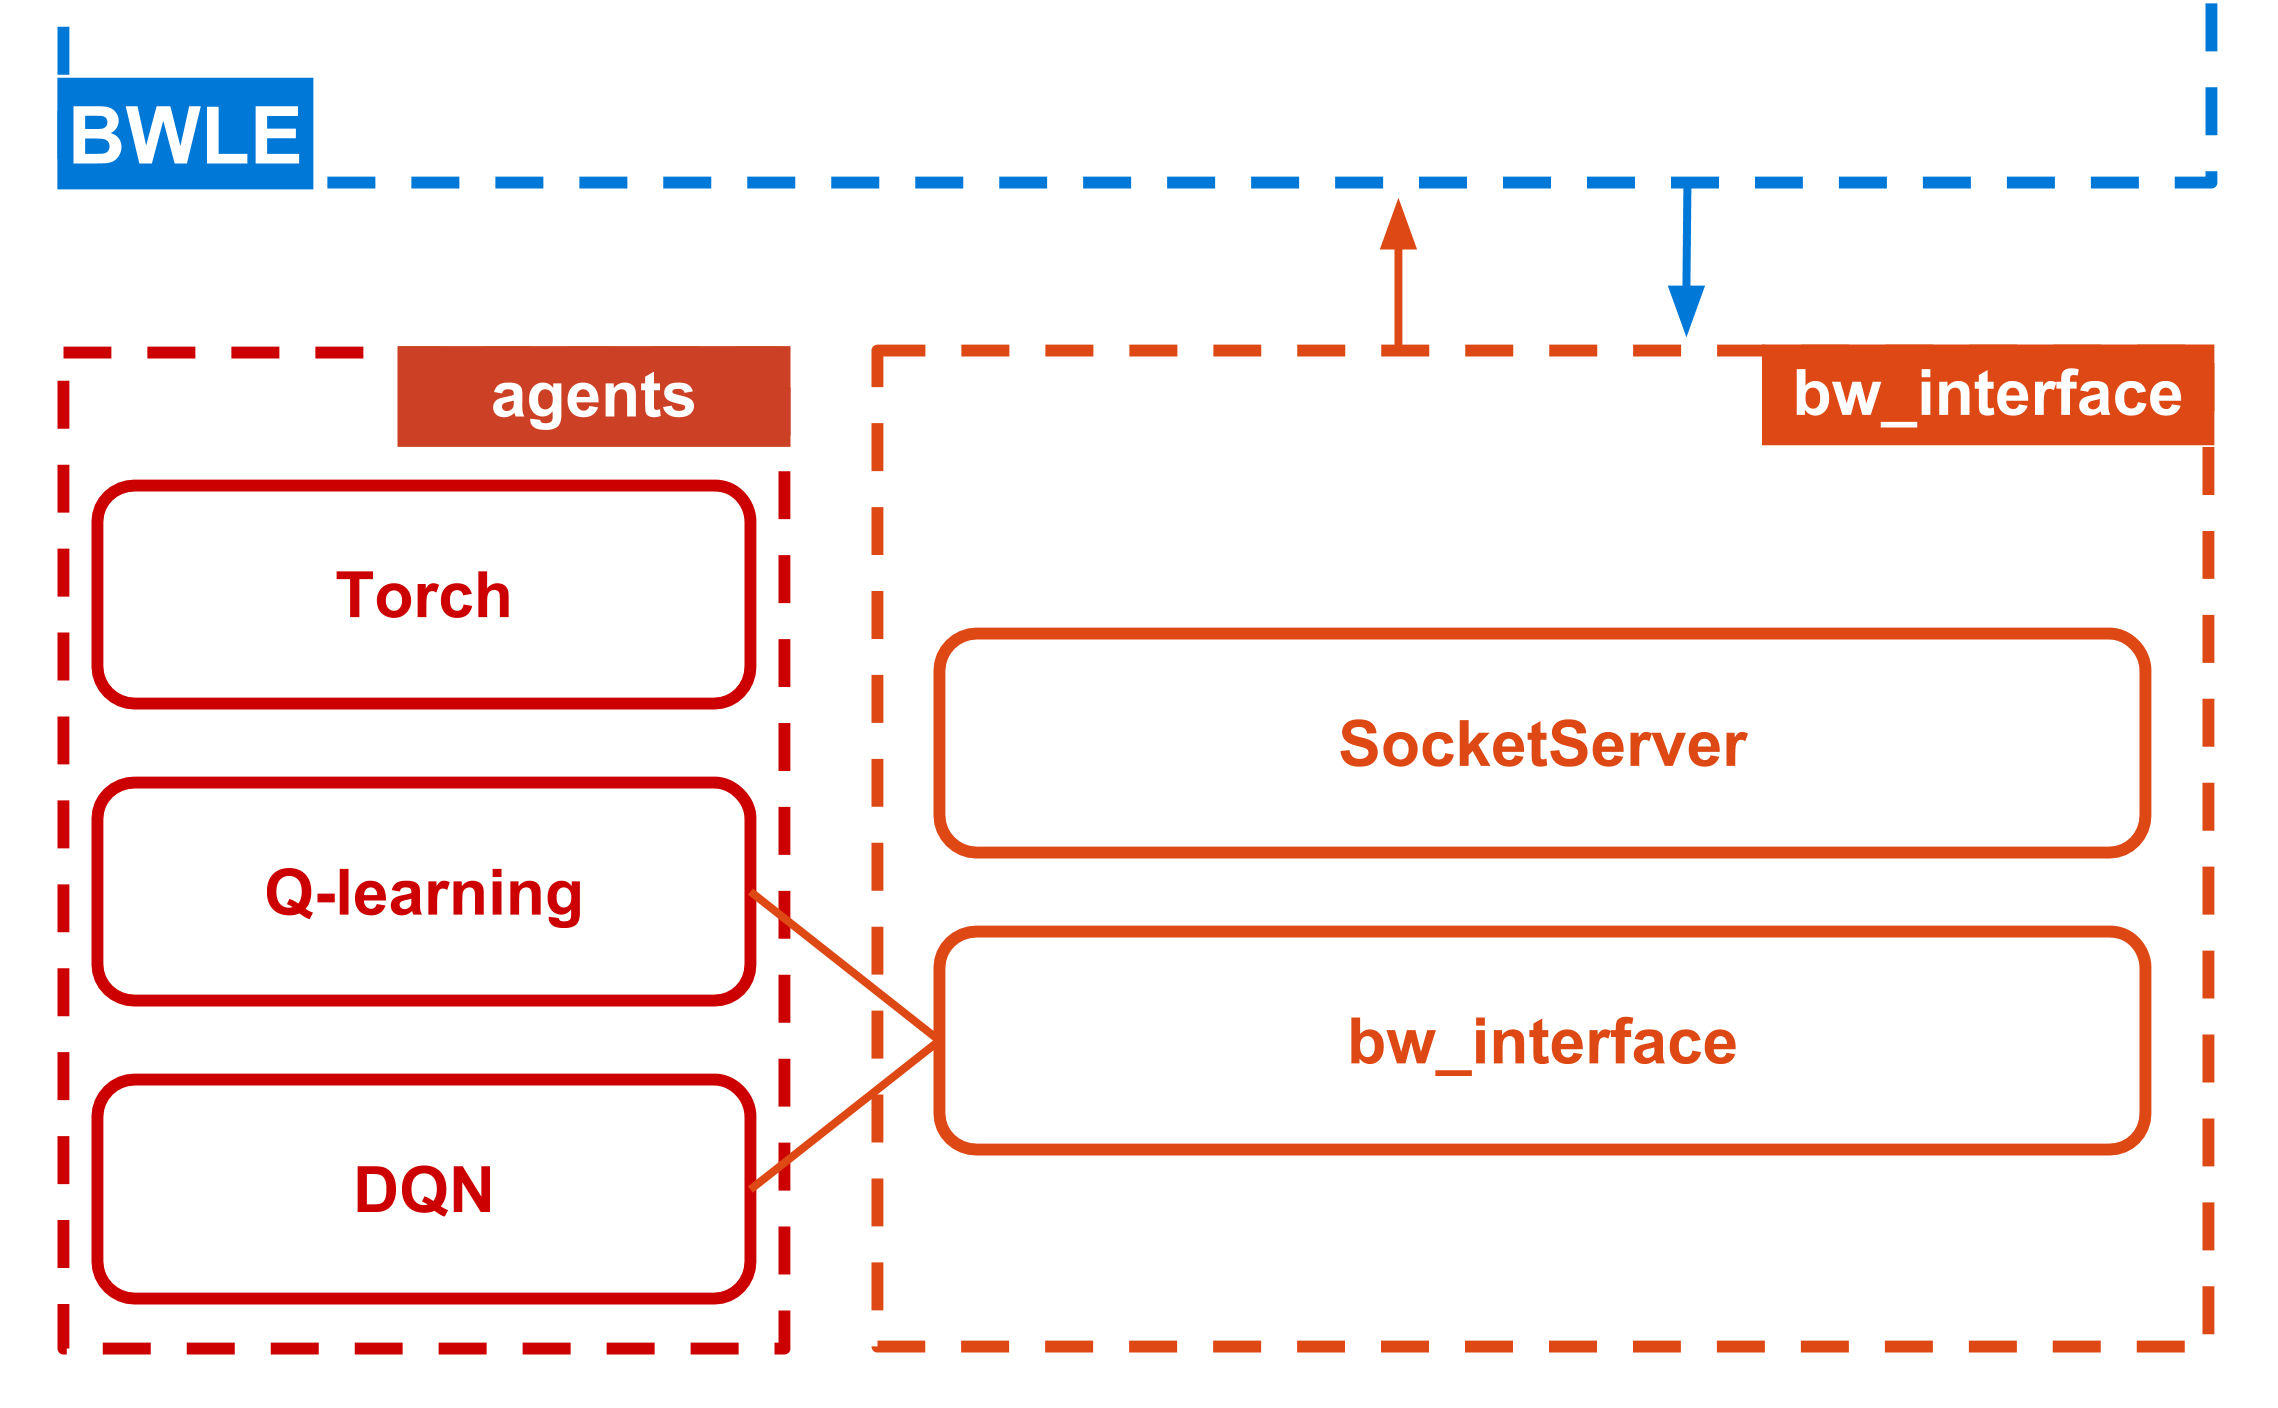
\includegraphics[width=\textwidth]{ch3/arch_linux}
    \caption{Overview of the architecture of the Linux sub-system.}
    \label{fig:arch_linux}
\end{figure}

We designed the Linux C++ interface to be complementary to the Windows client.
The interface started simply as a standard socket server and subsequently
evolved into a fully-fledged controller after adding a protobuffer parser, a
controller class and a storage system. Like the client, the server system
supports both synchronous and asynchronous modes, using non-blocking threaded
TCP sockets.

The overall system is coupled with the client and requires to update the
generated protobuffer interface every time the proto configuration file is
changed on the client side. Because of this we couldn't escape from adding the
library as a dependency, but this update was made painless by scripting the
whole process.

The system is split into three different modules:
\begin{description}
\item [Server] - Manages the connection with the client. It's the first object
  that the interfaces initialises, so it blocks the execution of the process
  until at least a client connects to it. The module was designed from the start
  to support multiple sockets and clients, but we didn't find the time to spin
  more than 2 instances of StarCraft on the cloud and run an heavy stress-test
  for this functionality.
\item [RingBuffer] - To provide a native way of storing and managing long-term
  information received from the client, we implemented a module to act as a
  middle-ware storage system based on a cyclic buffer. The history length can be
  changed when initialised and it's optimised so that the operation of switching
  data around the buffer is as fast as possible (this was done by doing some
  standard pointer manipulation).
\item [BotInterface] - This module essentially acts as the manager class for the
  whole interface. It starts the server, it initialises the data structures for
  the ring buffer and the temporary protobuf parser, and it provides methods to
  interact with the client.
\end{description}

Once we developed and tested the C++ interface, we had to create a LuaJIT
wrapper around it to allow our Lua agents to use it.

\subsubsection{Lua-compatible Interface}

LuaJIT provides an FFI library to wrap C/C++ objects and their interfaces
\citep{pall2008luajit}. The library provides a way to parse C declarations,
which can then be used to read a compiled shared object file containing the C
objects definitions. This allows to integrate C and C++ code (exported as C)
very quickly, without any need to manually write language bindings in Lua. The
Just-In-Time compiler generates instructions that are roughly as efficient
as the ones obtained by standard C compilers like GNU \texttt{gcc} and
\texttt{Clang}.

Arguably the most interesting part about our interface is that it provides a
method to take the raw pixel data sent by client and transform it into a Torch
tensor that can then be used by the Lua agents. This was possible by using the
Torch C API provided with the framework, which allowed us to copy the obtained
from the C heap to the LuaJIT storage system. We therefore became able to treat
our image as a Torch object and take advantage of the provided Torch
\texttt{image} library. We also leveraged the Torch \texttt{cunn} library to
make use of CUDA \citep{nvidia2008programming}, NVIDIA's GPU programming
library. This allowed us to train and test some of our agents on recent GPUs.

\subsubsection{Connecting the agents}

To provide the interface to the agent we used the FFI library to wrap the C++
objects, grouping the resulting functions into a class using Torch's
\texttt{Class} library. The end-result was \texttt{bw\_interface}, a module that agents could include
and use as a standard Lua table. 

We didn't wrap the entirety of the C++ functionality because we decided to
implement the ring buffer functionality in our agents as well, as to match the
common interface available to agents running on ALE for the sake of consistency.
The final accessible version of the interface to the agents ended up containing
a rich interface. Some important functions are for instance:

\begin{description}
\item [send\_packet(void)] - Sends the \texttt{ServerPacket} package to the
  client, allowing to control the execution of the environment.
\item [add\_action(int, int*)] - Takes a unit id and an array of action ids and
  adds it to the list of actions.
\item [get\_image\_tensor(void)] - Returns the last received image as a
  \texttt{DoubleTensor}. The tensor has been constructed in such a way to be
  directly compatible with the standard Torch \texttt{image} library. 
\item [get\_state(void)] - Return the game state as a hierarchical Lua table
  that the agent can walk through by simple recursive exploration of the
  attached dictionary of keys. The \texttt{inspect} library is used to test the
  state to check for possible errors.
\item [step(table, bool)] - In synchronous mode, order the client to update the
  game and perform a step. A step is defined as the amount of turns it takes to
  complete the defined set of actions (which can be a fixed amount).
\item [new\_game(bool)] - Order the game to start a new game and return the
  first state-reward pair.
\end{description}
 
\section{Summary}

In this chapter we have outlined the architecture of our entire system, looking
in particular at the design choices related to each module. We have described
our implementation and delineated some challenging issues when modelling RTS
games in a programmatic fashion.
